% Chapter 1

\chapter{State of the art}

\label{State of the art}

%PAPER of ref: https://www.researchgate.net/publication/286649850\_A\_survey\_of\_botnet\_detection\_based\_on\_DNS 
\section{Botnets}
%[A survey of botnet detection based on DNS]Kamal Alieyan Ammar ALmomani Ahmad Manasrah Mohammed M. Kadhum
As stated in the introduction botnets are an important problem for anyone involved somehow with the internet. Botnets can result in great economic damage. 

%Authority of Information Security. The 2016 Vietnam Information Security Report; Authority of Information Security, MIC: New York, NY, USA, 2016.
Botnets continuous improvement to become more resilient and powerful makes them an important threat to information security.

%http://dimva2014.isg.rhul.ac.uk/slides/phoenix-talk.pdf
Botnets can become very lucrative and can infect very large amounts of devices resulting in scary entities.
Here are some of these enormous entities: \textbf{Flashback} with 600k compromised targets, \textbf{Grum} with 840k compromised devices and sending 40 Billion spam emails per month, \textbf{TDL-4} with 4.5 Million victims in first the 3 months and \textbf{Gameover ZeuS} with 1 Million infections, because of its resilience mechanisms this botnet was one of the hardest to take down.\\

%source 6 (A survey of botnet detection based on DNS) 
The reason botnets are still an ongoing research topic is that there isn't a complete solution for their detection and mitigation. Researchers and organisations have to keep working to keep updated with all the new flavours criminals bring to the market.
\subsection{Definition}

%memoire1
%source Wielogorska, Monika and O'Brien, Darragh (2017) DNS Traffic analysis for botnet detection. In: 25th Irish Conference on Artificial Intelligence and Cognitive Science, 7-8 Dec 2017, Dublin, Ireland.
A botnet is a network of infected machines called bots, these bots owned and controlled by a remote attacker called the botmaster. Bots usually infect these machines without their owners' knowledge or consent
. The control of such bots is done through the Command and Control (CnC) server. The CnC server allows the master to issue commands to and receives responses from individual bots or aggregations of bots. These exchanges are done to update the software of the malware, execute attacks, exfiltrate data and more actions explained down below.

\paragraph{Bots} are small programs allowing to remotely control and perform commands on computers. They are the foundation of botnets. Their spreading mechanisms, infection and utilization are defined in the Botnet lifecycle in the structure section. These programs are embedded with port scanning, vulnerability scanning, exploitation and payloads that allow them to spread the botnet and infect their victims.\\
There are many different bots, some very modular such as the Agobot others simpler ones but easier to use such as the SDBot family. Bots families are also classified depending on the channel type and attack type, for example GT-Bots are a IRC bots. These 3 families are the most often found. Lesser usual ones have specific functions or plugins to fill in the gaps left by developers to customize the bots, a good examples would be the Dataspy Network X bots. There are very small bots such as the Q8 Bots and Perl-based bots that still allow for a large range of commands and attacks. Finally some bots are composed of a single file like kaiten bot which makes it very easy to upload to compromised machines.
%source http://www.honeynet.org/node/53

%source A survey of botnet detection based on DNS
In fact, botnets have specific characteristics as compared to other types of malware. For instance, the botmaster can control the infected machines and send commands without directly communicating with them. There are also a lot of bots working in a coordinated way and taking instructions from the botmaster to instantiate coordinated attacks.

%https://ccdcoe.org/cycon/2012/workshops/Intro_to_Botnets.pdf
% + source http://www.honeynet.org/node/52
Cybercriminals use botnets to execute a long list of malicious activities and structure related actions, we have listed some of these but any type of cyber attack can be uploaded to these bots and executed.\\

%source Emre Y (2011) A literature survey about recent botnet trends. http://geant3.archive.geant.net/Media_Centre/Media_Library/Media%20Library/botnet_trends_M2.pdf
Another reason botnets are a big threat is that criminals have started to provide botnets as a Service (BssS) which are considered a big part of the botnet economy. This popularised botnets to be used by anyone.

%memoire1
Because botnets are a large network of infected machines, they are able to carry out large scale attacks.\\ 
A victim host could be infected by targeting known vulnerability or by infected programs. When the victim is infected, the botnet will try to stay stealthy and with the exploit kit installed, it can do an extensive amount of damage. Here are some of the methods to control the infected hosts.
\begin{itemize}
\item Distributed Denial-of-Service Attacks. These attacks provoke a 
\item Spam email campaigns, 
\item Sniffing Traffic
\item Spy through Keylogging, file monitoring, 
\item Spreading new malware 
\item Installing Advertisement Addons and Browser Helper Objects (BHOs)
\item Google AdSense abuse
\item Manipulating online polls and games
\item Mass identity theft, stealing personal data such as mail accounts, intellectual property, military secrets, embarrassing information or bank credentials
%A Survey on Botnet Architectures, Detection and Defences
\item Secure the system(close NetBIOS shares, RPCDCOM)
\item host illegal sites
\item redirect traffic for the botnet
\item kill unwanted process running on the system
\item test for virtual machines and/or debugger software
\item add or delete auto-start applications
\item run or terminate programs
\item download and execute files
\item perform address and port scan
\item simulate key presses
\item Communicates with a handler or controller via public servers or other compromised systems. 
\item A botmaster commands bots to perform any of an number of different functions.
\item System of bots and controller(s) is referred to as a botnet or zombie network.

\end{itemize}



%http://www.technicalinfo.net/papers/PDF/WP_Botnet_Communications_Primer_(2009-06-04).pdf
A clear distinction between a bot agent and a common piece of malware lies within a bot’s ability to communicate with a Command-and-Control (CnC) infrastructure. CnC allows a bot agent to receive new instructions and malicious capabilities, as dictated by a remote criminal entity. This compromised host then can be used as an unwilling participant in Internet crime as soon as it is linked into a botnet via that same CnC.

% [Botnet Tracking Tools] SANS Institute 
The goals of an attacker in terms of bot recruitment can be categorized into two
broad categories. In the first case, the target of the attack is the computer that is being recruited. In the second case, the recruited bot is used to attack another target. Computers in a botnet are either the target of the attack, the perpetrator of the attack, or both. When bots are the perpetrator of the attack, the effectiveness of the attack is usually dependent upon the collective power of the botnet. Stated differently, the attacker is either after the valuable information on the computer or the storage, processing, and communication capabilities of the computer, or both. \\
The value of information on a personal computer is often overlooked. There are
many applications for home use, like tax preparation software, that store volumes of key personal and financial information. Browsers can cache website and account information. Email clients store contact information. Many home computers have sensitive work information on them, exposing a company's intellectual property to potential disclosure. These are just a few examples of the type of information that can be exfiltrated and abused by an attacker or sold to cyber criminals.\\A common botnet usage is the sending of spam emails. The spam emails can be used to carry malicious payloads in an attempt to infect the recipients of the spam emails. Spam can also be used to influence or manipulate user behavior such as the purchasing of advertised products, visiting of infected websites, or downloading of music or videos with malicious content.
Most cryptographic controls just buy the user time, in hopes that by the time the control is no longer good, the protected asset no longer has value. That is the theory behind password expirations. Password lifetime is set to be less than the time it takes to discover the password by brute force or other methods. The processing capabilities of a bot can be used for cryptanalysis purposes. Password cracking, brute force key discovery, and rainbow table creation are but a few examples. The collective power of a botnet greatly reduces the time a control is effective. Data storage is another bot resource an attacker can use without permission. Anonymity is important to the attacker, so storing ill-gotten gain across the botnet keeps incriminating evidence away from the attackers' machines. Additionally, there are efficiency, redundancy, and availability benefits from having a distributed data store. Ill-gotten gains can include personal information seized, pornography, intellectual property and malware.\\
Botnet rental has become a lucrative business. Botnets are rented and sold, usually for malicious purposes. Decentralized botnet architectures allow massive botnets to be partitioned into groups of smaller children botnets that can be parceled out for use and then reintegrated into the parent botnet after usage.
This paper will discuss botnet detection tools and techniques. This paper gives a brief introduction, a brief background on botnet characteristics, a summary of detection techniques, an overview of the BotMiner tool, reviews of two case studies where botnets were used to characterize behavior, and a conclusion.







\subsection{Structure}
\subsubsection{Life cycle}
Life cycles might differ from one bot to another but they have generally a common structure. This life cycle is composed of four steps
The exploitation/infection 


%A survey of botnet detection based on DNS
Botnet Lifecycle
exploitation phase: source 25,26,16
This is where the infection happens by exploiting a
vulnerability on the victim's host. Then the binary of the bot is downloaded onto the host. To find
this binary a DNS lookup has to be done. Which can't be avoided but can be hidden.
rallying source 18,27
attack execution source 17
update and maintenance source 6\\
Infection behavior 4 phases: 
%source Z. Zhu, G. Lu, Y. Chen, Z. J. Fu, P. Roberts, and K. Han, “Botnet research survey,” in 32nd Annual IEEE International Conference on Computer Software and Applications, pp. 967–972, Aug. 2008
1) Infection: vulnerability scanning \\
%source P. Barford and V. Yegneswaran, “An inside look at botnets,” in Advances in Information Security, vol. 27, pp. 171–191, Springer, Mar. 2007
2) Injection: exploited + download of bot's binary code\\ 
%source G. Gu, P. Porras, V. Yegneswaran, M. Fong, and W. Lee, “Bothunter: detecting malware infection through ids-driven dialog correlation,” in Proceedings of 16th USENIX Security Symposium on USENIX Security Symposium, pp. 1–16, Berkeley, CA, USA, 2007.
3) connection to the cnc and start to control the host\\
4) action on behalf of botmaster + maintain and upgrade periodically\\
For P2P 1 and 2 are similar but in 
% source 3) it uses a peer list instead to contact the initial peers +
searches until finds an alive peer 4) phase 1: update of peer list + download any available updates phase 2: starts malicious activities
based on STORM but similar for all P2P botnets 
% source S. Stover, D. Dittrich, J. Hernandez, and S.Dietrich, "Analysis of the storm and nugache trojans: P2p is here," The USENIX Magazine, vol. 32,
pp. 18-27, Dec. 2007.

\subsubsection{Channel}
TODO: after presenting the botnet structure we focus on the part where botmasters have turned their focus in evading detection and becoming more resilitent. In this section we want to discuss how the CnC channel works.

%J. Goebel and T. Holz, “Rishi: identify bot contaminated hosts by IRC nickname evaluation,” in Pro- ceedings of the first Conference on First Workshop on Hot Topics in Understanding Botnets, pp. 8, Berkeley, CA, USA, 2007.
Command and Control (CnC) CnC servers is what differentiates Botnets from other malware.

%https://ccdcoe.org/cycon/2012/workshops/Intro_to_Botnets.pdf
Means of receiving and sending commands and information between the botmaster and the zombies. Typical protocols: IRC, HTTP – HTTPS, DNS, etc\\
Protocols imply (to an extent) a botnet’s communication topology.
        The topology provides trades-off in terms of bandwidth, affectivity, stealth, and so forth.
        
TODO: explain the different techniques used to rally bots to an IP or a Domain (how do they regroup with master?)
% file:///D:/CyberSecurityMaster/Master%20Thesis/papers/Botnet_general/botnet_review.pdf
2.4.2 Command and Control Rallying Mechanisms
According to Choi et al. [20], botmasters want their bots
to be invisible but portable, therefore they use different
methods for bots rallying. They stated that not all bots
can have mobility and invisibility at the same time. They
described three rallying methods, namely; hard-coded IP
address, dynamic DNS, and distributed DNS.
In hard-coded IP address method; the bot binary has a
hard-coded IP address of its CnC server, the server can be
detected through reverse engineering, and the botmaster
can be quarantined or the botnet can be suspended. As
hard-coded IP address cannot be changed, this method
cannot provide mobility and does not make the botnet
invisible as well. On the other hand, in dynamic DNS
botnets migrate their CnC server frequently, upon the
instruction of botmaster. Using a list of servers provided
in the bot binary, a botmaster uses several CnC servers.
It uses dynamic DNS in order not to be detected or suspended,
and to keep the botnet portable. When connection
to the CnC server fails or shutdown, the bots will
perform DNS queries and will be redirected to a new CnC
server [2]. This redirection behavior of botnets is known
as “herding”. This method provides mobility and some
invisibility to the botnets. Finally, with distributed DNS,
botnets run their own distributed DNS service at locations
that are out of the reach of law enforcement. Bots
include the addresses of these DNS servers and contact
these servers to resolve the IP address of CnC servers
[2]. This method provides both mobility and invisibility
to their botnets.
In summary, while the hard-coded IP botnet makes
very easy for the newly infected nodes to join the botnet,
it also makes easy for law enforcement to track and
shutdown the botnet. On the other hand, using DNS to
migrate CnC servers make it harder for the newly infected
nodes to join the botnet. Some infected nodes might never
be able to join the botnet -in case they stay offline long
enough for all the addresses in the initial communication
list to be obsolete, however, it gives the botnet the flexibility
to hide its CnC severs.

Rallying mechanism %source H. Choi, H. Lee, H. Lee, and H. Kim, “Botnet detection by
monitoring group activities in dns traffic,” in The 7th IEEE International Conference on Computer
and Information Technology, pp. 715–720, Oct. 2007.
Objective for bots: invisible but portable -> different methods fo bot rallying: - ip hardcoded: the bot
binary has a hard-coded IP address of its CnC server, the server can be detected through reverse
engineering, and the botmaster can be quarantined or the botnet can be suspended. As hard-coded
IP address cannot be changed, this method cannot provide mobility and does not make the botnet
invisible as well.
dynamic DNS %source “Taxonomy of botnet threats,” white paper, Trend Micro Incorporated, Nov. 2006. (http://www.cs.ucsb.edu/ kemm/courses/cs595G/TM06.pdf)
botnets migrate their CnC server frequently, upon the instruction of botmaster. Using a list of
servers provided in the bot binary, a botmaster uses several CnC servers. It uses dynamic DNS in
order not to be detected or suspended, and to keep the botnet portable. When connection to the
CnC server fails or shutdown, the bots will perform DNS queries and will be redirected to a new
CnC server. This redirection behavior of botnets is known as “herding”. This method provides
mobility and some invisibility to the botnets.
distributed DNS 
%source “Taxonomy of botnet threats,” white paper, Trend Micro Incorporated, Nov. 2006. (http://www.cs.ucsb.edu/ kemm/courses/cs595G/TM06.pdf)
botnets run their own distributed DNS service at locations that are out of the reach of law
enforcement. Bots include the addresses of these DNS servers and contact these servers to resolve
the IP address of CnC servers. This method provides both mobility and invisibility to their botnets.

ME
The channel resilience of a botnet is critical to ensure good communication with the CnC server. It is a crtitical component of botnets, its failure is usually the end of the botnet's life. 



ME


[source]
%http://www.technicalinfo.net/papers/PDF/WP_Botnet_Communications_Primer_(2009-06-04).pdf

The ability for a bot agent to locate CnC infrastructure is a critical requirement for
maintaining control of the entire botnet for botnets that rely upon centralized CnC. If
the CnC cannot be found, a bot agent will not be able to receive new instructions.
While some bot agents may opt to function in an alternative autonomous “zombie”
mode – reverting to embedded instructions for propagation and infection – most bot
agents will continue to harvest local host information and poll the missing CnC at
regularly scheduled times.
Botnet Communication Topologies
Page 6
Botnet operators use a number of technologies to increase the probability that bot
agents will be able to locate the central CnC infrastructure. These tools and techniques
also make botnets more resilient to shut-down and hijacking maneuvers.
One key technology that enables CnC location resolution and failover resilience is
referred to as “fluxing”. Fluxing comes in two major flavors:
• IP Flux
• Domain Flux
Both technologies are used extensively by professional botnet operators


TODO: ways of securing their communication channel: encryption, rootkit and a number of DNS evasion techniques

\subsubsection{Topology}

[sources]\\
%[A Survey on Botnet Architectures, Detection and Defences] Muhammad Mahmoud, Manjinder Paul Nir, International Journal of Network Security · January 2014 file:///D:/CyberSecurityMaster/Master%20Thesis/papers/Botnet_general/botnet_review.pdf


%https://ccdcoe.org/cycon/2012/workshops/Intro_to_Botnets.pdf
Based on CnC channels, there are two typical botnet topologies:
Centralized
Decentralized (P2P)
     Traditional botnet metrics:
Resiliency
A botnet ability to cope with a loss of members (zombies) or servers
Latency
Reliability in message transmission
Enumeration
An ability to accurately estimate a botnet size
Difficulty for security analysis
Re-sale
A possibility to carve off sections of the botnet for lease or resale to
other operators. 

%http://www.technicalinfo.net/papers/PDF/WP\_Botnet\_Communications\_Primer\_(2009-06-04).pdf
Botnets come in all kinds of shapes and sizes. As a result, they employ a range of CnC
topologies in response to commercial defenses, legal shutdowns and hijacking
attempts. This evolution means that a criminal botnet operator has a number of wellstudied
CnC topology options to base a new botnet upon – each of which have
relative strengths and weaknesses

Botnet CnC topologies have been optimized to minimize network chatter and system
failures, just like commercial-grade technology tasked with remotely managing tens of
thousands of hosts. The precise CnC topology selected by a botnet operator often
reflects that individual’s perceived risk to continued command access and the financial
business model of that botnet

CnC topologies encountered in the wild typically match one of the following types:
• Star
• Multi-server
• Hierarchical
• Random

TODO: centralized vs decentralized botnets
TODO: metrics analyzed to choose best option: cf slide(11)(http://www.ijcttjournal.org/Volume4/issue-1/IJCTT-V4I1P104.pdf
TODO: present with visuals the different topologies and their purpose.

%source 
Modeling Botnets architectures:
diurnal propagation model %source D. Dagon, C. Zou, and W. Lee, “Modeling botnet
propagation using time zones,” in Proceedings of the 13 th Network and Distributed System
Security Sym- posium NDSS, 2006
Super botnet model % source R. Vogt, J. Aycock, and M. J. Jacobson, “Army of botnets,” in
Proceedings of Network and Distributed System Security Symposium (NDSS’07), pp. 111–
123, Reston, VA, USA, Feb. 2007
Stochastic P2P model %source E. Van Ruitenbeek and W. H. Sanders, “Modeling peer-to-peer
botnets,” in Fifth International Confer- ence on Quantitative Evaluation of Systems, pp. 307–
316, Sep. 2008 %source “The möbius tool,” Apr. 2011. (https://www.mobius.illinois.edu/)
advanced P2P hybrid model %source P.Wand, S. Sparks, and C. C. Zou, “An advanced hybrid
peer-to-peer botnet,” in Proceedings of the first Conference on First Workshop on Hot Topics
in Un- derstanding Botnets, pp. 2, Berkeley, CA, USA, 2007.

\paragraph{Star}
[source]
%http://www.technicalinfo.net/papers/PDF/WP\_Botnet\_Communications\_Primer\_(2009-06-04).pdf
The Star topology relies upon a single centralized CnC resource to communicate with
all bot agents. Each bot agent is issued new instructions directly from the central CnC
point. When a bot agent successfully breaches a victim computer, it is normally
preconfigured to “phone home” to this central CnC, whereupon it registers itself as a
botnet member and awaits new instructions.

    Pros 
Speed of Control
The direct communication between the CnC and the bot agent means that instructions (and stolen data) can be transferred rapidly
    Cons
Single point of failure
If the central CnC is blocked or otherwise disabled, the botnet is effectively neutered.\\
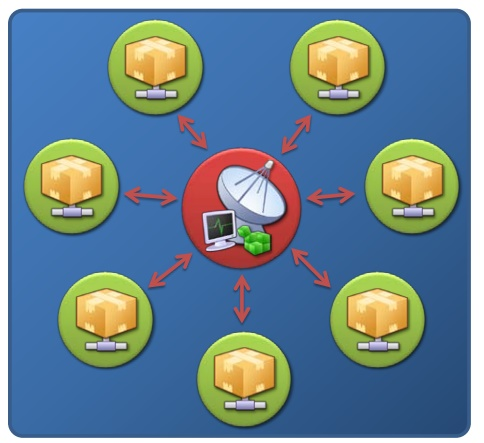
\includegraphics[scale=1]{img/star_topo.jpg}

%https://ccdcoe.org/cycon/2012/workshops/Intro_to_Botnets.pdf
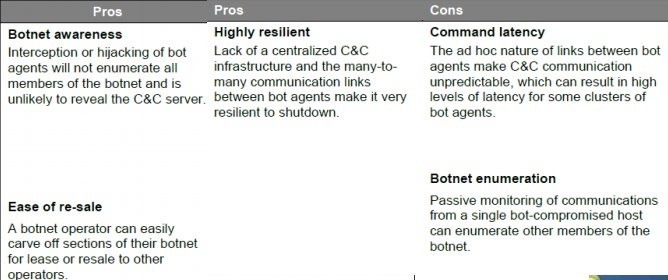
\includegraphics[scale=1]{img/centralized_topo}

\paragraph{Multi-server}
    Pros 
No single point of failure
Should any single CnC server be disabled, the botnet operator can still maintain control over all bot agents.
Geographical optimization
Multiple geographically distributed CnC severs can speed up communications between botnet elements.

    Cons
Requires advance planning
Additional preparation effort is required to construct a multi-sever CnC infrastructure.\\
\includegraphics[scale=1]{img/multi-server_topo.jpg}

\paragraph{Hierarchical}
    Pros 
  Botnet awareness
Interception or hijacking of bot agents
will not enumerate all members of the
botnet and is unlikely to reveal the CnC
server.
  Ease of re-sale
A botnet operator can easily carve off
sections of their botnet for lease or resale
to other operators.
    Cons
  Command latency
Because commands must traverse
multiple communication branches within
the botnet, there can be a high degree of
latency with updated instructions being
received by bot agents. This delay makes
some forms of botnet attack and
malicious operation difficult.

\paragraph{dynamic/P2P}
    Pros 
  Highly resilient
Lack of a centralized CnC infrastructure
and the many-to-many communication
links between bot agents make it very
resilient to shutdown.
    Cons
  Command latency
The ad hoc nature of links between bot
agents make CnC communication
unpredictable, which can result in high
levels of latency for some clusters of bot
agents.
  Botnet enumeration
Passive monitoring of communications
from a single bot-compromised host can
enumerate other members of the botnet

%http://dimva2014.isg.rhul.ac.uk/slides/phoenix-talk.pdf
\section{Use and abuse of DNS protocol}
%source A survey of botnet detection based on DNS
The current trend of botnets is to hide their channel using the DNS services to hinder their identification and rallying process.\\

\subsection{DNS}
%DNS
%-------
%Réexpliquer la base + présenter ds les requetes ce qui sera utilisé MAIS Principalement présenter la section réponse. 
%Différents types de records (qui sont utilisé ds la detection ou l'évasion donc les présenter.)
%Format utilisé pour le DNS OK
%-------
%Justifier le DNS passif comparé aux autres.

%A la place des discussion of features, placer la justification du choix de détéction en utilisant les études présentées. (je dois présenter toutes les autres techniques ss forcément aller en profondeur, comme ça on peut se positionner plus facilement.)

Most of the time users send DNS requests with a particular question for the DNS server. The server will the reply a DNS responses, similar to the request with the "answer" field filled with the information requested. Here is the structure of the packets transmitted to help with the understanding of the sections used as features later on.
\newpage
\subsubsection{Normal DNS message structure}
\begin{verbatim}
    +---------------------+
    |        Header       |
    +---------------------+
    |       Question      | the question for the name server
    +---------------------+
    |        Answer       | RRs answering the question
    +---------------------+
    |      Authority      | RRs pointing toward an authority
    +---------------------+
    |      Additional     | RRs holding additional information
    +---------------------+

\end{verbatim}

\subsubsection{Header section}
Here is a detailed description of the header of the DNS packets. 
\begin{verbatim}
	                               1  1  1  1  1  1
	 0  1  2  3  4  5  6  7  8  9  0  1  2  3  4  5
	+--+--+--+--+--+--+--+--+--+--+--+--+--+--+--+--+
	|                      ID                       |
	+--+--+--+--+--+--+--+--+--+--+--+--+--+--+--+--+
	|QR|   OpCode  |AA|TC|RD|RA| Z|AD|CD|   RCODE   |
	+--+--+--+--+--+--+--+--+--+--+--+--+--+--+--+--+
	|                QDCOUNT/ZOCOUNT                |
	+--+--+--+--+--+--+--+--+--+--+--+--+--+--+--+--+
	|                ANCOUNT/PRCOUNT                |
	+--+--+--+--+--+--+--+--+--+--+--+--+--+--+--+--+
	|                NSCOUNT/UPCOUNT                |
	+--+--+--+--+--+--+--+--+--+--+--+--+--+--+--+--+
	|                    ARCOUNT                    |
	+--+--+--+--+--+--+--+--+--+--+--+--+--+--+--+--+

\end{verbatim}

\begin{tabular}{l|l}
value & explanation \\
\hline
identifier & id of request\\
\hline
opcode & Operation Type: 0 $\rightarrow$ query, 1 $\rightarrow$ Inverse query, 2 $\rightarrow$ DNS status\\
\hline
aa\_flag & Authoritative Answer: response \\
\hline
tc\_flag & Truncation: flag set on truncated messages due to length greater\\ & than that permitted.\\
\hline
rd\_flag & Recursion Desired: if set, asks the NS to pursue query recursively.\\
\hline
ra\_flag & Recursion available: recursive query supported by NS\\
\hline
rcode  & Response Code: ignored in request, useful in answers to provide\\ & query information.(ex: type of errors)\\
\hline
questions\_count  & Number of entries in the Question section\\
\hline
answers\_count  & Number of RR in the Answer section\\
\hline
authority\_count  & Number of NameServer RR in the Authority section\\
\hline
additional\_count  & Number of RR in the additional section\\
\hline
\end{tabular}



\subsubsection{Question section}

\begin{verbatim}
                                    1  1  1  1  1  1
      0  1  2  3  4  5  6  7  8  9  0  1  2  3  4  5
    +--+--+--+--+--+--+--+--+--+--+--+--+--+--+--+--+
    |                                               |
    /                     QNAME                     /
    /                                               /
    +--+--+--+--+--+--+--+--+--+--+--+--+--+--+--+--+
    |                     QTYPE                     |
    +--+--+--+--+--+--+--+--+--+--+--+--+--+--+--+--+
    |                     QCLASS                    |
    +--+--+--+--+--+--+--+--+--+--+--+--+--+--+--+--+
\end{verbatim}

\begin{tabular}{c|l}
value & explanation\\
\hline
q\_name  & Domain name requested \\
q\_type  & Type of RR record requested \\
q\_class & Class of the request (often IN for internet) \\
\end{tabular}

\subsection{Botnets abusing DNS}
TODO: Present the different abuses of the DNS protocol to evade detection
(use previous descriptions but revisit writing and add more visualization and explanations on how exactly it works. (it is important for future arguments regarding the evasion methods. We need to inform our reader to be able to convince him later of our arguments)

Studies have shown that to avoid detection, botnets have been using multiple techniques utilizing the DNS protocol capabilities to reach their CnC. The DNS protocol has some features that have been exploited maliciously:  DNS tunnelling, fast-flux and domain flux.


%%-------------------------------- THIS IS WHERE WE EXPLAIN THE DIFFERENT TYPES OF EVASIONS ------------------------------------

TODO: Explain with the growing services of the internet "new"(research if they were part of the original protocol) capabilities arisen to allow this growth.(find an article supporting that). 
Explain Fast flux, domain flux and tunnelling used for legitimate purposes.
(find an article explaining how these are used by normal services or the standard of the protocol)



\subsubsection{Domain flux}
% explain  what domain flux is
Domain-flux is a type of flux where bots are equipped with a special Domain Generation Algorithm (DGA).
They use this algorithm to generate an ensemble of domains. The idea is to generate domains until one of them returns an IP address they can use to contact their CnC. The botmaster knows which domains are generated at a particular point in time and can register them before they are queried by
the bots to be reached. This improves the resilience of botnets infrastructure a lot.


TODO: present DF
[source]
%http://www.technicalinfo.net/papers/PDF/WP_Botnet_Communications_Primer_(2009-06-04).pdf

Domain Wildcarding 
abuses native DNS functionality to wildcard (e.g., *) a
higher domain such that all FQDN’s point to the same IP address. For example,
*.damballa.com could encapsulate both mypc.atl.damballa.com and
myserver.damballa.com. This technique is most commonly associated with
botnets that deliver spam and phishing content – whereby the wildcarded
information that appears random (e.g. “asdkjlkwer” of asdkjlkwer.atl.damballa) is 
Botnet Communication Topologies
Page 7
used by the botnet operator to uniquely identify a victim, track success using
various delivery techniques, and bypass anti-spam technologies.
• Domain Generation Algorithms 
are a more recent addition to bot agents. They
create a dynamic list of multiple FQDN’s each day, which are then polled by the
bot agent as it tries to locate the CnC infrastructure. Since the created domain
names are dynamically generated in volume and typically have a life of only a
single day, the rapid turnover makes it very difficult to investigate or block every
possible domain name.

   Location Resilience
Most botnets today rely upon DNS as the service for location of CnC infrastructure.
Fluxing DNS records provides varying degrees of resilience to shutdown and hijacking
that can be best summed up as:
Brittle: Single domain
Less brittle: Single flux
Resilient: Double flux
Very resilient: Domain flux


\subsubsection{IP flux}
IP flux or fast flux, 

%Survey on Botnets on DNS detection
Unfortunately, botnets use the DNS traffic as any other legitimate host, which makes differentiating the legitimate DNS traffic from the illegitimate one a very challenging problem [16]. Moreover,botnet owners attempt to hide their communication with the bots to obstruct any deployed botnet detection processes [17]. The attackers or botmasters use the DNS services to hide their command and control (CnC) IP address ;to make the botnet reliable and easy to migrate from server to another without being noticed

Fast-Flux Service Network (FFSN) allows for one domain name to have an unlimited number of IP addresses, short TTLs(Time to live) values and the IPs rotating in a round robin fashion. IP addresses belonging to such a domain act as a proxy for any device attempting a connection with their respective
CnC server. This process helps botnet controllers avoid detection and blacklisting. But can be confused with real traffic. It has a different categories:
\begin{enumerate}
\item Single-flux: Multiple IP addresses are assigned to the same domain (either CNAME or A records). (low TTL, multiple autonomous system(AS) locations, proxies for master)
\item NS flux: Multiple NS records assigned to the same domain
\item Double-flux: Multiple name servers are assigned to the same domain and then use single-flux for the multiple IP addresses of the master. This provides a second layer of redundancy. This also means that the TTLs are short for the A records and the NS records too.
\end{enumerate}

[source]
% file:///D:/CyberSecurityMaster/Master%20Thesis/papers/Botnet_general/botnet_review.pdf
Normal FF\\
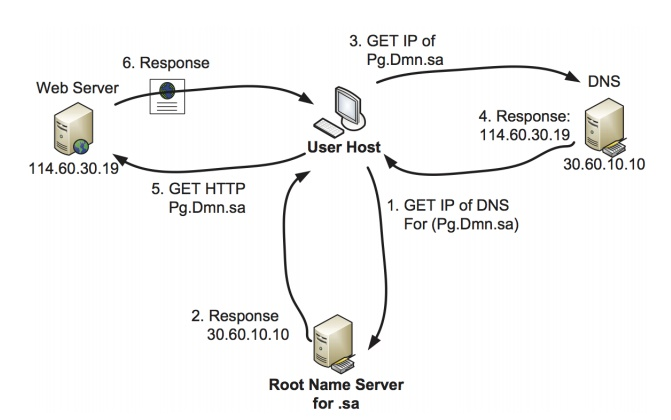
\includegraphics[scale=.7]{img/normal_FF.jpg}
single flux\\
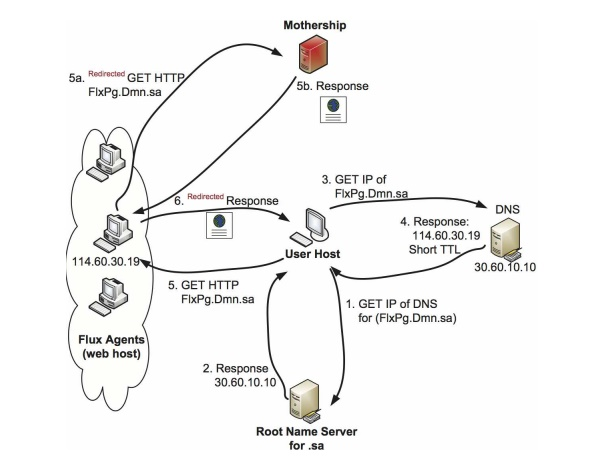
\includegraphics[scale=.7]{img/single_FF.jpg}
double flux\\
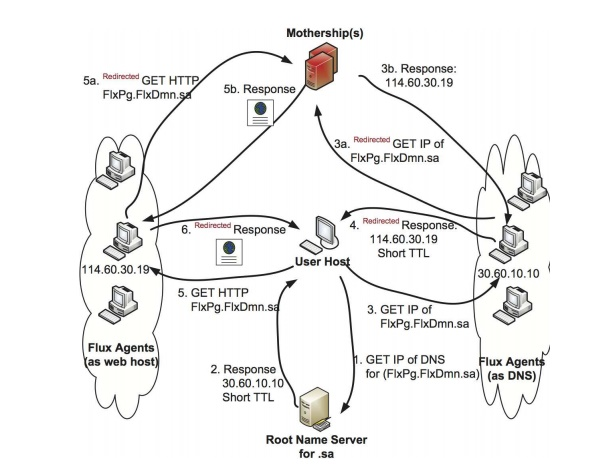
\includegraphics[scale=.7]{img/double_FF.jpg}

%source P. B¨acher, T. Holz, M. K¨otter, and G. Wicherski,“Know your Enemy: Tracking Botnets,” Oct. 2008. (http://www.honeynet.org/papers/bots)
This is done to allow the botnet’s domain name to have multiple IP addresses. In the meantime,
involved DNS records are constantly changing every few minutes using a combination of round robin
IP addresses and a very short TTL from any given particular DNS resource record.
In FFSN, the victim client first sends an address query to DNS. Then, the DNS returns the IPs of a
subset of active flux-agents. After that, the flux-agent relays the client’s request to the mothership3.
The key factor in FFSN is the combination of a very short TTL and the round-robin answer from a
large pool of active agents
%source P.Wand, S. Sparks, and C. C. Zou, “An advanced hybrid peer-to-peer botnet,” in
Proceedings of the first Conference on First Workshop on Hot Topics in Un- derstanding Botnets, pp.
2, Berkeley, CA, USA, 2007.
Some features for FF detection: nb of A records returned: 1-3 normal, 5 or more ff nb of NS: normal
-> small, ff -> several NS + several A records for the NS AS: small nb of A from 1 AS -> normal,
located in different AS -> ff Hardware and IP: range of IP is diverged -> ff No physical agent -> ff no
garantee uptime.
FIGURE NORMAL FF AND BAD FF (single and double)

DNS is an Internet service which translates names of sites into their numeric IP addresses. For
every host, DNS has a list of A records each with a given Timeto- Live (TTL) value (normally from 1
to 5 days). DNS returns these A records in round-robin way.
CDN use a lower TTL to provide their content more efficiently
Fast-Flux Service Network (FFSN) is a distributed proxy network -built on compromised machines
(flux-agents)- that direct incoming DNS requests to the botnet’s desired address on the fly.
%source J. Nazario and T. Holz, “As the net churns: Fast-flux botnet observations,” in The 3rd International Con- ference on Malicious and Unwanted Software, pp. 24– 31, Oct. 2008.



\subsubsection{DNS tunnelling}
DNS tunnelling implies the act of tunnelling other protocols or data through DNS, for example using the TXT as q\_type and using the requests to actually send data. This has been done to avoid restrictions but is now also used to hide malicious traffic from botnets. They can also use DNS tunnelling to remain undetected while exfiltrating data. \cite{Botnet1}

\subsubsection{Maybe Domain shadowing (need more research)}
%[A Review Paper on Botnet and Botnet Detection Techniques in Cloud Computing] Shahid Anwar, Jasni Mohamad Zain, Mohamad Fadli Zolkipli, Zakira Inayat! Conference: ISCI 2014, September 2014
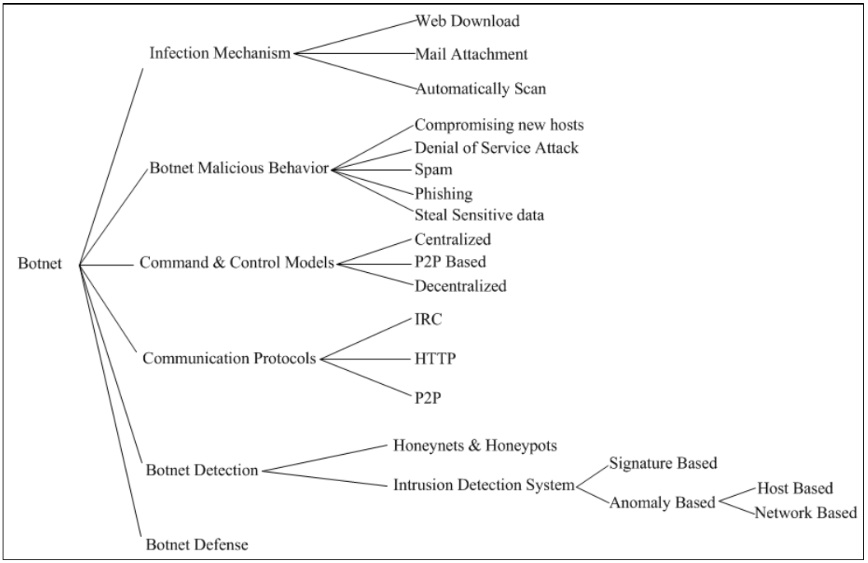
\includegraphics[scale=.8]{img/botnet_taxonomy.jpg}


\section{Botnet detection related papers}
\subsection{classification of botnet research and detection}
In this section related to papers focused on Botnet detection, we are going to present the classifications of botnets and what part of the research we have decided to focus on.

%[Botnet Detection Based On Machine Learning Techniques Using DNS Query Data]
A number of botnet, detection measures, such as honeynet-based and Intrusion Detection System (IDS)-based, have been
proposed. However, IDS-based solutions that use signatures seem to be ineffective because recent
botnets are equipped with sophisticated code update and evasion techniques

Botnet detection and defence
Early bots detected through signature 
%source “SNORT,” Mar. 2006. (https://www.snort.org/)
-> vulnerable to any new botnet, but useful for old ones

%source D. Plohmann, E. Gerhards-Padilla, and F. Leder, “Botnets: measurement, detection, disinfection and defence,” in ENISA Workshop (Giles Hogben, ed.), Mar. 2011. botnet detection
classification: passive and active
%source “Taxonomy of botnet threats,” white paper, Trend Micro Incorporated, Nov. 2006. (http://www.cs.ucsb.edu/ kemm/courses/cs595G/TM06.pdf)
3 types of behavior: 
- network based behavior: observable network traffic between botmaster and bots, can be used to detect individual bots and their CnC server. 
- host based beavior: observable calls on the systems infected by botnets. 
- global correlated behavior: global behavior characteristics, structure will be similar to current structures; same for all mechanisms
%source H. Choi, H. Lee, H. Lee, and H. Kim, “Botnet detection by monitoring group activities in dns traffic,” in The 7th IEEE International Conference on Com- puter and Information Technology, pp. 715–720, Oct. 2007. 

"4.1.3 DNS Traffic Botmaster use DNS rallying to make their botnets invisible and portable. Choi et
al. [20] proposed botnet detecdetection mechanism by monitoring their DNS traffic. According to the
authors, bots use DNS queries either to connect or to migrate to another CnC server. The DNS
traffic has a unique feature that they define as group activity. Bots can be detected by using the
group activity property of botnet DNS traffic while bots are connecting to their server or migrating
to another server. There are three factors that help in distinguishing botnet DNS queries from
legitimate DNS queries [20]; (1) queries to CnC servers come only from botnet members (fixed IP
address space size), (2) botnet members migrate and act at the same time, which leads to temporary
and synchronized DNS queries, (3) botnets usually use DDNS for CnC servers. For a botmaster to
keep its bot hidden and portable, it relies on DNS to rally infected hosts. In botnets, DNS queries
can appear for many reasons. They appear during rallying process after infection, during malicious
activities like spam or DoS attacks, during CnC server migration, during CnC server IP address
change, or after CnC server or network link failure. Based on the aforementioned five situations of
DNS query used in botnets, the authors have developed a Botnet DNS Q Detection algorithms, which
distinguishes the botnet. This algorithm starts by building a database for DNS queries comprised of
the source IP address, domain name and timestamp. Then, they group DNS query data using the
domain name and timestamp field. After that, they remove redundant DNS queries. Finally, botnet
DNS queries are detected using a numerically computed some similarity factor [20] This algorithm
cannot detect botnets migrating to another CnC server. Therefore, they developed a Migrating
Botnet Detection algorithm by modifying the botnet DNS query detection algorithm. Similarly, this
algorithm starts by building a database for DNS queries comprised of the source IP address, domain
name and timestamp. Then, it groups DNS query data using the domain name and timestamp field.
After that, it removes redundant DNS queries. The next step will be to compare IP lists of different
domain name with same size of IP list, because bots use two different domain names for the CnC
server during migration [20]. These algorithms are protocol and structure independent and are
capable of detecting unknown and encrypted botnets. However, these are not for real-time
detections and have low accuracy for small networks. Furthermore, they are very sensitive to
threshold values which need to be chosen very carefully to balance false positives and false negative
rates.


% ========================================================================================

%source Botnet_Detection_Based_On_Machine_Learning_Techniques_Using_DNS_Query_Data
Honeynet: capture and analyze Pros: Easy to build, low ressources requirements Cons: Hard to
scale, limited interactions + can be reverted by hackers to learn new evasion techniques.
IDS: monitor and look for signs 2 types: signature or anomaly based through DNS analysis(most
promising) %source [ Botnet Detection Technology Based on DNS] Xingguo Li , JunfengWang ,and Xiaosong Zhang 
%source [A survey of botnet detection based on DNS] Kamal Alieyan • Ammar ALmomani • Ahmad Manasrah • Mohammed M. Kadhum
Anomaly detection approaches that work: 
- DNS Blacklist (for malware, botnets and spambots) 
%source [Revealing botnet membership using DNSBL counter-intelligence] Ramachandran, A.;Feamster, N.; Dagon, D.*
- detect botnets when they try to communicate with their CnC:
NXDomains 
%source: Villamari-Salomo, R.; Brustoloni, J.C. Identifying botnets using anomaly detection techniques applied to DNS traffic.
%source http://citeseerx.ist.psu.edu/viewdoc/download?doi=10.1.1.131.1318&rep=rep1&type=pdf
- recursive DNS queries detecting botnet related services %source: Perdisci, R.; Corona, I.; Dagon, D.; Lee, W. Detecting malicious flux service networks through passive analysis of recursive DNS traces
- DGA 
1) Main DGA %source: Yadav, S.; Reddy, A.K.K.; Reddy, A.; Ranjan, S. Detecting algorithmically generated malicious domain names. 
2) Decision tree + Bayes for DGA classification 
%source: Stalmans, E.; Irwin, B. A framework for DNS based detection and mitigation of malware infections on a network
- Kopis = high level DNS query analysis (upper hierarchy)
%source: Antonakakis, M.; Perdisci, R.; Lee, W.; Vasiloglou, N., II; Dagon, D. Detecting malware domains at the upper NS hierarchy
- Exposure 
%source Bilge, L.; Kirda, E.; Kruegel, C.; Balduzzi, M. Exposure: Finding Malicious Domains Using Passive DNS Analysis
graph analysis 
%source Jiang, N.; Cao, J.; Jin, Y.; Li, L.; Zhang, Z.L. Identifying suspicious activities through DNS failure graph analysis.
- reputation system 
% source Manos Antonakakis, Roberto Perdisci, David Dagon, Wenke Lee, and Nick Feamster. Building a Dynamic Reputation System for DNS



%======================================================================================


ME
TODO: In the beginning we explain the detection classification proposed by the large survey. Then we explain what we have researched and how we'll use it in our work. Keep in mind that it isn't a list of papers, it is a list of information that will be used or not later in the paper, that has to cover that topics current research state and that we need to argue on reasons we want to keep articles or not and what information we'll use.
\\\\
After this presentation on the techniques used by Botmaster to set their botnets into certain topologies and evading the best they can current detection systems. We are now presenting the research papers that have tried to detect botnets using this different evasion techniques. Since the end goal is to find the best features for an all-in solution, we have structured the current state of research as follows: 
First we will present the current all-in solutions that exist, the features they extract and what model they have created. 
Secondly, to achieve our goal towards improving these solutions, the objective is to find better features and better models. We will present studies focused on single detection models that cover the field of detection through passive DNS analysis. For each study we will list the features proposed, understand their purpose and do a first selection if a thorough comparison has been made with the features presented. Otherwise they will saved for further analysis.
\\\\
In a recent survey of the state of the art regarding Botnet detection based on DNS traffic analysis\cite{survey}, they present a classification of botnet techniques (A survey of botnet detection based on DNS). They divide the classification into 2 categories, the honeynets and IDS(Snort). The later having evolved the most and where we want to focus. Most IDS were for a long time using signature-based techniques(check the IDS section for more details, p6). These are effective but only work with known botnets. Because they are signature-based there is a need to keep a blacklist updated very often, because a simple change creates a new signature and would be undetected if the database isn't updated with the latest signatures.\\
Newer techniques, described as "anomaly based" have emerged for 2 reasons: to detect unknown botnets and to respond to the new type of evasions that followed. Botnets have become a lot more resilient and stealthy. It has pushed the research to focus on features that would allow to distinguish between benign and malicious traffic.
These new researches capable of detecting new bots are divided into 2 sections: host-based and network-based. This means anomalies focusing on a single host or the traffic of a network. The host-based research focused on detecting bots in single hosts by monitoring local processes and kernel level routines.(BotSwat) The big problem of these propositions were the inability to scale them, we would need large monitoring system on each host with complex capabilities to communicate with each other and do correlation(EFFORT framework, the only one apparently. Do a bit more research on this framework and correct any mistakes in its previous description). This is what the second section aims to solve by monitoring networks. This activity can be done passively by simply collecting the traffic and analysing it (passive monitoring) or actively by injecting packets into the network forged to make the bots react, and then analyse the network response. 
Active monitoring: explain in more detail the rest of the approaches.
The part that our study focus on because "explain a valid reason for this part having more weight then the other ones, explain that our study could be a model combining different steps of the classification."
Finally explain the different passive approaches: 
\\
Explain that these passive detection can also be divided into specific counters for certain evasion systems such as DF, FF, tunnelling. Or be put together in an all-in solution to detect botnets independently of the evasion technique used.
\\
The first step in the research was to find the models that would be the current baseline for all-in solutions: Here we can start with 2 already gathered ones, and used the survey papers to find all-in solutions (if there are more than EXPOSURE), present them completely (features, dataset, model, purpose). 
IDEA: use the survey study chart to show strengths and weaknesses of papers.
\\
- Step needed before presentation of these papers:
classify them into the folders, 
create a summary for each one with the following information:
Model (data processing, dataset used, classification process, features)
finally for each relevant paper either do a summary with the 4 components or simple summary if redundant information.


After this part we are supposed to be done with the research, we have a last discussion of how the following step is planned and what information from this chapter will be translated into the rest of the thesis.
ASK: should we introduce the research on datasets in the SOTA or the model presentation?
ME
\subsection{All-in solutions}
\subsubsection{Exposure}
[source]
%[EXPOSURE: a Passive DNS Analysis Service to Detect and Report Malicious Domains] Leyla Bilge, Symantec Research, France Sevil Sen, Hacettepe University, Turkey Davide Balzarotti, Eurecom, France Engin Kirda, Northeastern University, USA Christopher Kruegel, University of California - Santa Barbara, USA.

\quote{EXPOSURE, a system that employs large-scale, passive DNS analysis techniques to detect domains that are involved in malicious activity. They use 15 features extracted from DNS traffic.}\\

\paragraph{Time-based}
When we analyse many requests to a particular domain over
time, patterns indicative of malicious behaviour may emerge.\\
These were supposed to be the features with the most weight, unfortunately due to lack of the same caliber of capture available to the authors of Exposure, we could not test out the 4 features related to time. Either because the datasets are compositions of smaller datasets, or because the timestamps are too short.
\paragraph{DNS answer based}
Here are some domain-flux features: A domain name can map to multiple IP addresses. In such cases,the DNS server cycles through the different IP addresses in a round robin fashion and returns a different IP mapping each time. \\
Malicious domains typically resolve to compromised computers that reside in different locations. The attackers typically use domains that map to multiple IP addresses, and IPs might be shared across different domains.
\begin{itemize}
\item the number of different IP addresses that are resolved for a given domain during the experiment window
\item the number of different countries that these IP addresses are located in
\item the reverse DNS query results of the returned IP addresses
\item the number of distinct domains that share the IP addresses that resolve to the given domain (false positive can be reduced with google reverse DNS which will have hosting providers in top answers)
\end{itemize}
\paragraph{TTL value based}
Low TTL and Round-Robin DNS: \\
\begin{itemize}
\item high availability (Content Delivery Networks (CDNs))
\item botnets using this, makes them resistant to DNS Blacklists(DNSBL) and take downs. Often using Fast-Flux Service Networks (FFSN).
\end{itemize}
Because FFSN are usually detectable because of low TTL and growing list of distinct IP addresses for a domain, it explains the purpose of the TTL features.
\paragraph{Domain name based}
Finally 2 simple features to expect detection of DGA: there is a big difference between legit domain names and domains generated by DGAs(Domain Generation Algorithms(DGAs).

This can be noticed with 2 simple features:\\
\begin{itemize}
\item ratio numerical chars to length of domain name
\item length of the longest meaningful substring to length of domain name
\end{itemize}
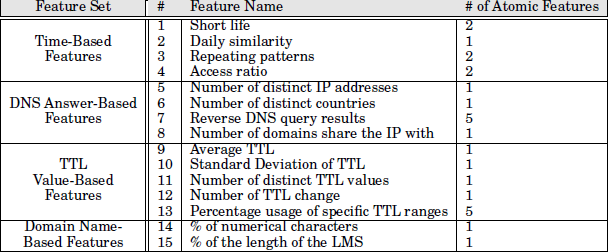
\includegraphics[scale=.3]{img/exposure_features.png}

\subsection{Possible approaches to provide better features}
\subsubsection{Domain-flux}
TODO: domain-flux can is mostly about analyzing domain names, here is a list of papers that attempt to do that with different metrics and features:  
%Detecting domain-flux botnet based on DNS traffic features in managed network Dinh-Tu Truong and Guang Cheng. https://de.wikipedia.org/wiki/Domain\_Flux, https://www.sciencedirect.com/science/article/pii/S1742287614001182, https://blog.malwarebytes.com/security-world/2016/12/explained-domain-generating-algorithm/\\
DGA specific\\
Detecting Algorithmically Generated Malicious Domain Names, %http://dimva2014.isg.rhul.ac.uk/slides/phoenix-talk.pdf

%memoire
%%%%%%%%%%%%%%%%%%%%%%%
Domain flux is mainly used with DGAs and so here are some papers that have proposed an approach to detect it.

In \cite{dga}, they analyse the basic features that are common to most domain generated by DGA. The first is the length that can be an identifier because DGAs have long domain name. Recent DGAs have shown to have shorter lengths to blend with the other domains. They then propose 3 primitive features that capture linguistic and structural characteristics. They end with 2 more advanced features that cover the shortcomings of the primitive ones. They propose these features to detect DGAs:\\\\
\begin{tabular}{|l|}
\hline
length of the domain name excluding TLD (top level domain)\\
\hline
Number of vowels in the Second Level Domain (SLD)\\
\hline
Number of consonants in the SLD\\
\hline
Number of digits in the SLD\\
\hline
SLD trigram entropy\\
\hline
SLD trigram conditional probability\\
\hline
\end{tabular}
\\

These 6 features are very simple but have obtained really good results. The reason for the last 2 features is to improve the quality of the classification since some of the features could belong to botnets or legit domains. The definition of the features is explained in the section where this approach is analysed.

In this paper\cite{dga3}, they propose an unsupervised approach based on anomaly detection with a set of metrics analysing ngrams of the SLD. They use the Kullback-Liebler divergence measure with unigrams and bigrams, they also used the Jaccard index between bigrams and the last feature is the Edit distance. These 3 features are used widely in the DGA detection research because of their efficiency. \\

In this paper\cite{dga4}, they realize that during the generation algorithm, most of the domains will not be up, this will generate a lot of NXDomain responses. Furthermore, the caching of NXDomains is limited which means that they cannot hide this traffic. Their contribution consists of a clustering technique based on domain names and request patterns; and similarity metrics for malicious domains detection. What can be retrieved from this study is the feature related to NXDomains, and the clustering process for big datasets.

In \cite{phoenix}, they explain the shortcomes of some of the other approaches. The study works in 2 phases: DGA discovery and DGA detection. In the discovery phase they apply the following filters that focus on linguistics: percentage of meaningful word in the domain name; popularity of the ngrams of the domain. They construct a base generated with the top 100.000 domains from Alexa. Then they define a distance (Mahalanobis distance) and thresholds(loose and stric ones) to determine when domains can be considered DGAs. They use known malicious domains to determine their thresholds. Afterwards they propose a sytem to cluster DGAs. They create a graph where each node is a domain and edges are created if both nodes resolve to similar IPs, the weight is proportional to the number of common resolved IPs. From all the "communities" discovered, they extract different common features to be reintroduced in the detection phase for each family of DGAs.
%%%%%%%%%%%%%%%%%%%%%%%%%%%%%%%%%%%%%%%%%%%
\subsubsection{Fast-flux}
%memoire
%%%%%%%%%%%%%%%%%%%%%%%%%%%%%%%%%%%%%%%%%%
For IP flux, most papers have similar features they propose to detect fast-flux. The big challenge is to find the small differences and detect malicious fast-flux networks(FFSN) from content delivery networks(CDNs). Both use fast-flux for different reasons such as load balancing, high availability and evasion.\\
The features most papers \cite{honeynet}\cite{ff2}\cite{ff3}bring forward are shown on the figures below\cite{ff_botconf}, and listed here:\\\\
\begin{tabular}{|l|}
\hline
Numerous unique A records for a domain\\
\hline
Numerous unique NS records for a  domain\\
\hline
Different Autonomous Systems (ASN) for the IPs of linked to the same domain\\
\hline
Different countries for the IPs of linked to the same domain\\
\hline
Short Time-To-Live (TTL)\\
\hline
\end{tabular}
\\\\\\
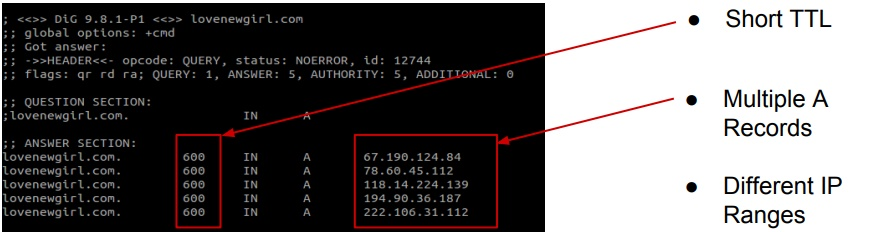
\includegraphics[scale=.7]{img/ff_features.jpg}\\
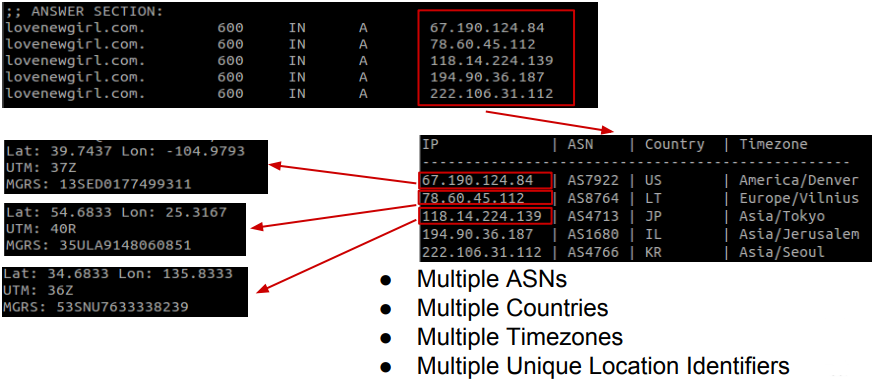
\includegraphics[scale=.6]{img/ff_features_2.png}
\\We present now the different features and approaches proposed to distinguish the CDNs from FFSN.\\

Before the approach taken by \cite{ff2}, most of the detection was based on DNS Blacklisting (DNSBL), their new approach was a passive analysis of recursive DNS traffic. Recursive DNS  when your query is send to your DNS server, it starts by checking its cache and then will recursively ask other DNS servers until finding the address. Their purpose was to allow direct analysis of DNS requests and detect malicious ones. They want to improve the HoneyNet\cite{honeynet} features(short time-to-live (TTL), set of resolved IPs returned at each query changes rapidly, usually after every TTL, the overall set of resolved IPs obtained by querying the same domain name over time is often very large, the resolved IPs are scattered across many different networks)\\
They start by applying filters to cluster the different networks of FF using the list above. On these clusters they then applied statistical supervised algorithms to do the classification. They used a base of features provided by \cite{fluXOR} and added their own. \\It starts with the passive features: \\\\
\begin{tabular}{|l|}
\hline
Number of resolved IPs\\
\hline
Number of domains (in a cluster = domains with similar IPs)\\
\hline
Avg. TTL per domain in a cluster\\
\hline
Network prefix diversity = ratio between the number of distinct\\ /16 network prefixes and the total \\
\hline
number of IPs (measures the scattering)\\
\hline
Number of distinct domain names that resolved to at least one of \\the IP addresses in the considered cluster\\
\hline
IP Growth Ratio. This represents the average number
of new IP\\ addresses discovered per each DNS response related to any domain\\
\hline
\end{tabular}
\\\\
Then the active ones:\\\\
\begin{tabular}{|l|}
\hline
Autonomous System (AS) diversity (ratio between the number of distinct\\ ASs where the IPs of a cluster reside and the total number of resolved IPs. \\Same for the following diversities)\\
\hline
BGP prefix diversity\\
\hline
Organization diversity\\
\hline
Country Code diversity\\
\hline
Dynamic IP ratio (ratio of dynamic vs total IPs using keywords in reverse\\ DNS lookups)\\
\hline
Average Uptime Index (average uptime for the IPs in a cluster,\\ Uptime tested through probing)\\
\hline
\end{tabular}
\\\\
They use these features on a Decision Tree classifier (efficient, easy to interpret and auto pruning of useless features) to classify malicious and legit FF networks.\\

In the following paper\cite{ff3}, they propose some novel features compared to the other papers. To avoid redundancy, only the features not explored in previous papers will be detailed. In the paper they present the restrictions FFSNs face compared to CDNs: FFSN cannot choose the location which makes the IP address very scattered and no Uptime garantee. Possible distinctions: the lack of control results in number of unique A records returned different and the number of NS records in a single lookup (because the NS can be hosted inside the FFSN and return many NS records whereas legitimate CDNs return a very small set of NS records). The IP diversity restriction brings another feature which is the number of unique ASNs. Legitimate CDNs tend to return a single ASN for all their A records where FFSN are dispersed.\\
They decide not to include TTLs as a feature because both CDNs and FFSN have low TTLs. Finally,  they introduce functions of the different features above to classify FFSN and CDNs.\\
\textbf{Fluxiness} is the total of unique A records for a domain divided by the number of A records returned for each lookup. This measures consistency in the unique A records returned. \\
\textbf{Flux-score} an hyperplane that separates benign from malicious fast flux where $ x = (n_A,n_{ASN},n_{NS})$ (unique A records, ASN and SN records) and the plane is defined as follows\\
%\begin{equation}
%F(x) = 
%\begin{cases}
%	w^Tx-b > 0  & \text{x is a FFSN}\\
%	w^Tx-b \leq 0 & \text{x is CDN}\\
%\end{cases}
%\end{equation}
From $F(x)$ they induce a metric $f(x) = w^Tx$ with w the weight of the vector and b a bias. $f(x) > b$ would mean x is a FFSN. By empirically testing this on a labelled dataset they determined the value of w and b. $w = (1.32,18.54,0)$ and $b =142.38$. We can notice that $n_{NS}$ does not have any impact. It could be argued that FFSN will try to mimic CDNs to have the same metrics, but as argued earlier, the metrics used take into account the restrictions FFSN have. The rest of the study approaches the detection of FFSN using the HTML content returned by the spam websites.\\

%Detection of Fast-flux Networks using Various DNS Feature Sets
This paper\cite{ff5} regroups the large majority of features encountered in the other papers accompanied with to some novel additions resulting a long list of 16 features: \\\\
\begin{tabular}{c|l}
Type & Features\\
\hline
 & Number of unique A records\\
DNS Answer-based &  Number of NS records\\
 & DNS packet size\\
 & TC (Tnmcated) Flag is set\\
\hline
 & Edit Distance\\
Domain name-based & KL (Kullback-Leibler) Divergence (unigrams and bigrams)\\
 & Jaccard Index (unigrams and bigrams)\\
\hline
 & Time Zone Entropy of A records\\
Spatial-based & Time Zone Entropy of NS records\\
 & Minimal service distances (mean and standard deviation)\\
\hline
 & Number of distinct autonomous systems\\
Network-based & Number of distinct networks\\
 \hline
 & Round Trip Time of DNS request\\
Timing-based & Network delay (mean and standard deviation)\\
& Processing delay (mean and standard deviation)\\
& Document fetch delay (mean and standard deviation)\\
\end{tabular}
\\

%%%%%%%%%%%%%%%%%%%%%%%%%%%%%%%%%%%%%%%%%%%%%

\subsubsection{DNS tunnelling}
%memoire
%%%%%%%%%%%%%%%%%%%%%%%%%%%%%%%%%%%%%%%%%%%%%%%
In \cite{tunn1}, use of TXT RR with segmented and encrypted data.
Rdata features: we look for the Shannon entropy of the strings. Measures the randomness of the string. Since encrypted data as a high level of entropy this is one of the things we'll be looking for. We are looking for "high byte entropy".Because of inherent reasons this entropy for a small string can't reach the max, we are looking at the "statistical byte entropy" instead.

The complete list of features for the Rdata:
\begin{itemize}
\item number of distinct byte values in m
\item minimum byte value in m
\item maximum byte value in m
\item number of ASCII capital letters (byte values 65-90) in m
\item number of ASCII digits (byte values 48-57) in m
\item length of m in bytes
\item absolute difference of the statistical byte entropy at given length of m and the entropy of m
\item size of all Rdata messages
\end{itemize}
They expect these behavioural communication features to be effective enough in order to extend a classifier based on the rdata features.
\\\\
In this paper\cite{tunn}, they propose a visual approach to detecting DNS tunnelling, by plotting the following features, you can detect by "visual anomaly detection" the presence of DNS tunnelling. The features are:
\begin{itemize}
\item x-axis: destination IP
\item y-axis: character count
\item radius: hostname length
\item colour: request type
\end{itemize}


%(cf Detecting DNS tunnelling)
%DNS has been used as a communication method by malware. Known malware
%using DNS include: Feederbot (Dietrich, 2011) and Moto (Mullaney, 2011). Both of
%these malware examples use DNS TXT records for command and control.
%%%%%%%%%%%%%%%%%%%%%%%%%%%%%%%%%%

\subsubsection{Behavioral}




